\section{Operation on Exascale Hardware}

The ECP's exascale platforms are unique in many ways.
The previous section summarized the major software development hurdles faced when preparing for the platforms.
This section describes further technical challenges in compiling and executing \vtkm.

%% \ken{
%%   Each subsection should be roughly 1/2 page.
%%   (1 page total.)
%%   The subsection shold start with a brief overview of the system, focusing on unique features.
%%   The following paragraphs should describe a challenge and then discuss how the challenge was addressed.
%%   Some examples include long compile times, errors for function pointer calls, compiler errors.
%%   The section should end with a paragraph summarizing the current state of \vtkm on the system.
%% }

\subsection{Frontier}
Frontier was the first system delivered under the ECP program. Deployed at the Oak Ridge Leadership Computing Facility (OLCF), Frontier is also the first system to achieve exascale by hitting 1.19 exaflops on the High-Performance Linpack benchmark.
Frontier is an AMD-based system with 9,472 AMD Epyc CPUs (with 9,408 reserved for compute only) totalling over 600,000 cores.
However, the majority of the processing power comes from 37,888 AMD MI250X GPUs (with 37,632 reserved for compute only) totalling over 8.3 million cores.
The system is organized into 74 racks, each comprising 64 blades with 2 nodes each.
A node consists of a single CPU and 4 GPUs with 4 TB of RAM.
Each GPU consists of two Graphics Compute Dies (GCD), which means that a node presents itself to device code as having 8 GPUs.
That leaves us with a total count of 75,776 GCDs (with 75,264 reserved for compute only).

Porting to a new system that is also under active development brings many challenges.
When the pre-exascale development systems for Frontier became available, \vtkm frequently broke the compiler.
At one point in the build, test, and release cycle for the compilers, AMD had the \vtkm team building the compilers from bleeding-edge source to help debug the crashes.

As the compilers stabilized, the team discovered another issue---astronomically long compile times.
As an anecdote for a particularly long compile time, \vtkm development switched over to a second system when it came online.
A week later, the system administrators for the pre-exascale systems contacted us to ask if they could kill a compile job because it was consuming all the memory on the login node.
It turned out that a \vtkm compile was still running on the initial system more than a week later.
More commonly, \vtkm would take 20 hours to completely compile.
The team would work with AMD to test a new compiler, and the cycle would begin anew.
Thankfully, these compile-time issues have been corrected.
Currently, a full build of \vtkm with tests and benchmarks can be completed on Frontier in under 20 minutes.

Along the way there were many issues that required solutions from AMD, Kokkos, and the \vtkm teams. Some examples are as follows:
\begin{itemize}
\item \emph{Compiler Errors.}
  \vtkm uses template metaprogramming \citep{Meyers2005}.
  Although this code is fully C++14 compliant, it sometimes flexes the compiler in unexpected ways and may cause internal compiler errors.
  Resolving these issues requires dialog with the compiler engineers.
\item \emph{Optimizer Internal Looping.}
  In addition to compiler fixes, certain portions of the code found the compiler optimizing the code too aggressively in extended internal loops.
  Hints were added to prevent the compiler from optimizing out of control.
  Furthermore, the \vtkm source was broken into smaller units to reduce template instantiation and to reduce compiler resource utilization, as described in the \nameref{sec:filter-overhaul} section.
\item \emph{Degradation of Sorting Parallelism.}
  The original Kokkos sorting algorithm had not accounted for \vtkm workloads that used integral types (e.g., sorting keys).
  A binning algorithm that worked well for uniformly distributed values degraded to a largely serial process when many values landed in a single bin.
  A simple fix by the Kokkos team provided a $12\times$ speedup in these workloads.
\item \emph{Function Pointers Unsupported on AMD GPUs.}
  \vtkm was modified over several months to remove all calls through function pointers as part of the removal of virtual methods (as described in the \nameref{sec:virtual-methods} section).
\end{itemize}

\begin{figure}[htb]
  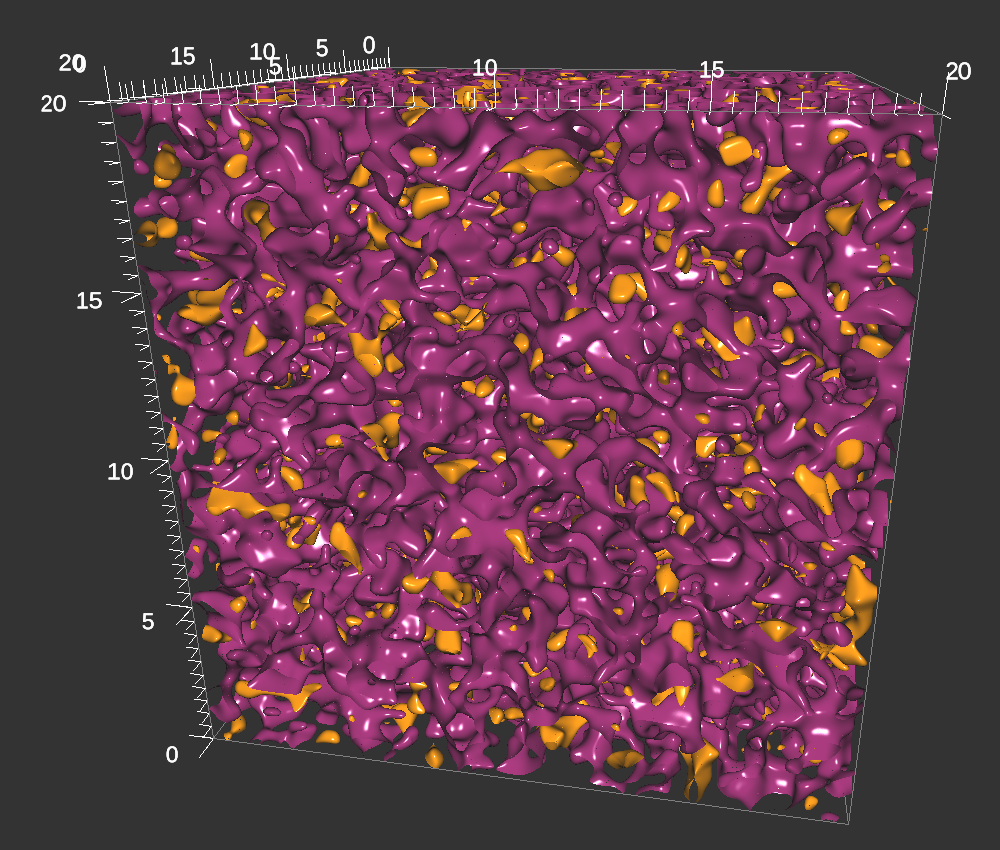
\includegraphics[width=\linewidth]{frontier-render-clip}
  \caption{
    Output from \vtkm scaling study that demonstrated rendering at full scale on the Frontier supercomputer.
  }
  \label{fig:frontier-render}
\end{figure}

When Frontier became available to the various code teams, the \vtkm team at the University of Oregon undertook an experiment to establish \vtkm's scalability.
The team created Perlin noise data comprising 80 trillion cells and distributed for a full-system run that used 9,400 nodes and 74,088 GPU GCDs.
The total time to render this dataset was 300~ms.
Figure~\ref{fig:frontier-render} shows an example output from this test.

%\markb{De-snarkified. It's so vanilla now.}
%\ken{Hey, lots of people like vanilla.}

\subsection{Aurora}

%\assign{Silvio}

The Aurora supercomputer is deployed at the Argonne Leadership Computing Facility (ALCF) and is expected to deliver over 2 exaflops of computational power. With 166 racks and 10,624 nodes, it boasts 21,248 Intel Xeon Max Series CPUs and 63,744 Intel Data Center Max Series GPUs.

Our journey on Aurora began in August 2020 when we started building \vtkm on the Joint Laboratory for System Integration's test platform at Argonne National Laboratory.
We began our work using the Iris test platform, which consisted of 20 nodes equipped with Intel Gen 9 GPUs.
By September 2021, we transitioned to the Arcticus test bed, which featured 17 nodes equipped with 2$\times$ Intel Server GPUs code-named Arctic Sound.
In August 2022, we conducted tests on the Florentia test platform, which contained early versions of the Aurora GPUs.
Finally, by January 2023, our efforts shifted to Sunspot, the Aurora test and development system, which had 128 nodes with 2$\times$ Intel Xeon Max Series CPUs and 6$\times$ Intel Data Center Max Series GPUs.
The first light on Aurora occurred in August 2023.

Throughout our porting and testing efforts, we maintained close collaboration with Intel engineers and ALCF performance engineering staff. This collaboration led to the identification and resolution of several bugs in successive versions of the Intel oneAPI software development kit. In November 2020, we completed a first set of early \vtkm benchmarks on Iris by using Kokkos with OpenMP target offload. However, in February 2021, we encountered issues with virtual methods when transitioning to Kokkos with SYCL. Fortunately, the team anticipated this problem and had already started the process of replacing virtual methods (see the \nameref{sec:virtual-methods} section), and this issue was resolved soon after. Additionally, we worked with Intel to address long build times.

By December 2023, the latest \vtkm and Kokkos development branches were successfully running on Aurora and achieving a 97\% success rate in regression testing. Porting, deployment, and integration efforts are set to continue on Aurora as we move beyond the ECP era.
